\section{Vertex periods}\label{sec:periods}

\Cref{thm:finite-normal} turns a global minimizer into a normal vertex period: a normal
Pontryagin extremal whose control is a vertex of the simplex on each of finitely many pieces
(\cref{def:vertex-representation,def:normal-period}). On a piece of constant vertex control the
state, the frame and the costate solve linear differential equations with constant
coefficients, so everything that happens along the piece is given by explicit formulas in a few
numbers at its start. A period is then described by finitely many numbers, related by algebraic
and logarithmic identities, and the maximum principle becomes a list of sign conditions on
them. This section collects these formulas and conditions, which the case analysis of
\cref{sec:reverse,sec:short-runs,sec:forward,sec:mixed,sec:smaller-short} uses, and states the
theorem that reduces the problem to periods with at most five pieces.

Throughout, $P$ is a normal vertex period with $N$ pieces, switching times $\tau_k$, labels
$i_k\in\Z/3$ and terminal time $T$, indexed by $k\in\Z$ through the twist
$\tau_{k+N}=\tau_k+T$, $i_{k+N}=i_k+1$ (\cref{def:vertex-representation}). Its state $X$, frame
$g$, costates $\Lambda_1,\Lambda_R$ and cost multiplier $\lambda=-1$ are those of
\cref{def:normal-period}. We write $m_k(j)=p_j(X(\tau_k))$ for the margins at the switch
$\tau_k$ ($0\le k\le N$). Since $p_j(R^{-1}XR)=p_{j-1}(X)$ and
$X(T)=R^{-1}X(0)R$, the rule
\begin{equation}\label{eq:per-margin-twist}
  m_{k+N}(j)=m_k(j-1)
\end{equation}
extends them consistently to all $k\in\Z$. The \emph{active
margin} of piece $k$ is $a_k=m_k(i_k)$, the margin of its own vertex at its start, and its
\emph{factor} is
\[
  q_k=\exp\bigl(2(\tau_{k+1}-\tau_k)/a_k\bigr)>1,
\]
so that the piece lasts $(a_k/2)\log q_k$. Both sequences are
$N$-periodic. We also write
\[
  s_k=a_k+a_{k+1},\qquad K_k=a_k^2+4.
\]

\subsection{One piece of constant control}\label{sec:per-one-arc}

For a label $i$ and $w>0$ let
\[
  T_i(w)=\frac{w+w^{-1}}{2}\,I+\frac{\sqrt3\,(w-w^{-1})}{2}\,Z_{\ee_i}
\]
be the \emph{tangent factor} of the vertex $\ee_i$. Since $Z_{\ee_i}$ is traceless with
determinant $-1/3$, $Z_{\ee_i}^2=I/3$, and $T_i(w)$ is the exponential of a multiple of
$Z_{\ee_i}$: $T_i(w)T_i(v)=T_i(wv)$, $\det T_i(w)=1$, $T_i(w)^{-1}=T_i(w^{-1})$ and
$R^{-1}T_i(w)R=T_{i+1}(w)$.

\begin{lemma}[One piece]\label{lem:one-arc}
Let $(g,X)$ be a state trajectory on $[0,T]$ whose control is the vertex $\ee_i$ almost
everywhere on $(s_0,s_1)\subset[0,T]$, and let $(a,b,c)=(p_i,p_{i+1},p_{i-1})(X(s_0))$. For
$t\in[s_0,s_1]$ put $w=\exp((t-s_0)/a)$ and $q=w^2$. Then
\begin{enumerate}[label=\textup{(\alph*)}]
\item $X(t)=T_i(w)^{-1}X(s_0)T_i(w)$, and the tangent frame $V=gX$ satisfies
  $V(t)=V(s_0)\,T_i(q)$;
\item the margins at time $t$ are
  \begin{equation}\label{eq:per-one-arc}
    p_i=a,\qquad p_{i+1}=(a+b)q-a,\qquad p_{i-1}=\frac{a+c}{q}-a;
  \end{equation}
\item with $q=\exp(2(s_1-s_0)/a)$, the cost of the piece is
  \begin{equation}\label{eq:per-arc-cost}
    -\frac32\int_{s_0}^{s_1}\ip{J}{X(t)}\,\dd t
    =\frac{\sqrt3}{4}\,a\bigl((a+b)(q-1)+(a+c)(1-q^{-1})-a\log q\bigr).
  \end{equation}
\end{enumerate}
For a normal vertex period this gives, for every $k\in\Z$,
\begin{gather*}
  m_{k+1}(i_k)=a_k,\qquad m_{k+1}(i_k+1)=\bigl(a_k+m_k(i_k+1)\bigr)q_k-a_k,\\
  m_{k+1}(i_k-1)=\frac{a_k+m_k(i_k-1)}{q_k}-a_k,
\end{gather*}
and the cost $\cost(T,X)$ of the period is the sum of~\eqref{eq:per-arc-cost} over the pieces
$0\le k<N$.
\end{lemma}

\begin{proof}
The margin $p_i$ is, up to a factor, the trace pairing with $Z_{\ee_i}$, and
$\ip{Z_{\ee_i}}{[Z_{\ee_i},X]}=0$. Along the piece $P_{\ee_i}(X)=Z_{\ee_i}/\ip{Z_{\ee_i}}{X}$ is a
multiple of $Z_{\ee_i}$, so $p_i$ is constant and $P_{\ee_i}(X)=-(\sqrt3/a)Z_{\ee_i}$ is a constant
matrix. The state equation $X'=[P,X]$ then has the solution
$X(t)=e^{(t-s_0)P}X(s_0)e^{-(t-s_0)P}$, and $e^{(t-s_0)P}=T_i(w)^{-1}$. The margins of this
conjugate are a direct computation. Writing
$g(t)=h(t)e^{-(t-s_0)P}$, the frame equation becomes $h'=h\,(X(s_0)+P)$ with a constant
traceless matrix, whose exponential is explicit. Uniqueness of Carath\'eodory solutions
identifies the actual trajectory with this flow, also when the control differs from $\ee_i$ on
a null set. Integrating $-\frac32\ip{J}{X}=\frac{\sqrt3}{2}(p_0+p_1+p_2)$ with~\eqref{eq:per-one-arc} gives~\eqref{eq:per-arc-cost}.
\end{proof}

Each margin stays positive along a piece, so a piece with factor $q$ is admissible exactly when
$1<q<1+c/a$: the margin of the label $i-1$ decreases and must not reach $0$. We call $i+1$ the
\emph{growing} label and $i-1$ the \emph{decreasing} label of the piece.

The margins at a switch lie on the quadric $m_k(0)m_k(1)+m_k(1)m_k(2)+m_k(2)m_k(0)=4$
(\cref{lem:margins}), and two of them are active margins: at $\tau_k$ the label $i_{k-1}$ has
margin $a_{k-1}$ (it was constant along piece $k-1$) and the label $i_k$ has margin $a_k$. The
third margin is therefore $(4-a_{k-1}a_k)/s_{k-1}$, and the update rule of \cref{lem:one-arc}
expresses each factor through the active margins alone.

\begin{lemma}[Factors from active margins]\label{lem:per-factors}
For every $k$, according to the signs of the switches before and after piece $k$
(\cref{def:signs} below),
\[
  \begin{array}{llll}
    \text{forward, forward:} & q_kK_k=s_{k-1}s_k, &\qquad
    \text{reverse, forward:} & q_ks_{k-1}=s_k,\\[2pt]
    \text{reverse, reverse:} & q_ks_{k-1}s_k=K_k, &\qquad
    \text{forward, reverse:} & q_ks_k=s_{k-1}
  \end{array}.
\]
\end{lemma}

\begin{proof}
Consider two forward switches. The label $i_k-1=i_{k-1}$ of the previous piece has margin
$a_{k-1}$ at $\tau_k$, so the growing label has margin $b=(4-a_{k-1}a_k)/s_{k-1}$ and
$a_k+b=K_k/s_{k-1}$. The next piece has the growing label, so
$a_{k+1}=(a_k+b)q_k-a_k$ and $s_k=K_kq_k/s_{k-1}$. The other three cases are the same
computation with the roles of the growing and the decreasing label exchanged.
\end{proof}

Up to the labels, a period is therefore determined by its signs and its active margins, subject
to $q_k>1$ and $a_ka_{k+1}<4$. At a turn, $q_k>1$ reads $a_{k+1}>a_{k-1}$ after a reverse switch
and $a_{k+1}<a_{k-1}$ after a forward one. The cost takes a symmetric form in these variables.
Let
\[
  G(a,b)=3ab-4-(a^2+b^2)\log(a+b)+\tfrac12a^2\log(a^2+4)+\tfrac12b^2\log(b^2+4),
\]
and
$G_a(a,b)=\partial G/\partial a
=3b-2a\log(a+b)-\frac{a^2+b^2}{a+b}+a\log(a^2+4)+\frac{a^3}{a^2+4}$.

\begin{lemma}[Signed action]\label{lem:per-signed-action}
With the switch signs $\varepsilon_k\in\{\pm1\}$ of \cref{def:signs},
\[
  \frac{8\,\cost(T,X)}{\sqrt{12}}=\sum_{k=0}^{N-1}\varepsilon_k\,G(a_k,a_{k+1}).
\]
\end{lemma}

\begin{proof}
Write the cost~\eqref{eq:per-arc-cost} of piece $k$, times $4/\sqrt3$, with the margins of
\cref{lem:per-factors}. It splits as $\varepsilon_kF_1(a_k,a_{k+1})+\varepsilon_{k-1}F_1(a_k,a_{k-1})$, a
term for the switch after the piece and one for the switch before it, with
\[
  F_1(a,n)=a\Bigl(n-\frac{4-an}{a+n}\Bigr)-a^2\log(a+n)+\frac{a^2}{2}\log(a^2+4).
\]
The two terms that belong to the switch $k$ add up to
$\varepsilon_k\bigl(F_1(a_k,a_{k+1})+F_1(a_{k+1},a_k)\bigr)=\varepsilon_kG(a_k,a_{k+1})$.
\end{proof}

The derivative of the sum in \cref{lem:per-signed-action} with respect to one active margin
$a_k$, the others fixed, is $\varepsilon_{k-1}G_a(a_k,a_{k-1})+\varepsilon_kG_a(a_k,a_{k+1})$. This quantity
reappears in the stationarity identity (\cref{lem:stationarity}).

\subsection{The tangent closure}\label{sec:per-closure}

The tangent frame $V=gX$ is multiplied on the right by $T_{i_k}(q_k)$ along piece $k$
(\cref{lem:one-arc}(a)). It starts at $V(0)=X(0)$ and ends at $V(T)=R\,R^{-1}X(0)R=X(0)R$, and
$X(0)$ is invertible. This gives one matrix equation that every period satisfies.

\begin{lemma}[Tangent closure]\label{lem:tangent-closure}
The factors and labels of a normal vertex period satisfy
\[
  T_{i_0}(q_0)\,T_{i_1}(q_1)\cdots T_{i_{N-1}}(q_{N-1})=R.
\]
\end{lemma}

The closure is simplest in the \emph{triangular coordinates} $Y\mapsto CYC^{-1}$,
$C=\left(\begin{smallmatrix}\sqrt3&1\\\sqrt3&-1\end{smallmatrix}\right)$, in which
\begin{gather*}
  T_0(q)=\begin{pmatrix}q&0\\0&q^{-1}\end{pmatrix},\qquad
  T_1(q)=\begin{pmatrix}q^{-1}&q-q^{-1}\\0&q\end{pmatrix},\\
  T_2(q)=\begin{pmatrix}q^{-1}&0\\q^{-1}-q&q\end{pmatrix},\qquad
  R=\begin{pmatrix}0&1\\-1&1\end{pmatrix}.
\end{gather*}
The change of coordinates
has $\det C=-2\sqrt3<0$: it reverses orientation, which matters for the sign of ellipticity in
\cref{sec:per-casimir}. The labels, the factors and the margins at the switches, related by the
update rule of \cref{lem:one-arc} and by the closure read from every switch, are all that
\cref{sec:terminal} needs to solve the closure for $N\le5$.

\subsection{Switch signs and the five classes}\label{sec:per-classes}

Neighbouring labels differ, and labels live in $\Z/3$, so each switch either advances the label
by one or moves it back by one.



The margin of the growing label increases along a piece, so a forward switch hands the control
to the vertex whose margin has just grown, and a reverse switch hands it to the vertex whose
margin has just decreased. Both kinds occur in extremals, but they behave differently: runs of
reverse switches carry the first-order obstructions of \cref{sec:reverse}, while the forward
switches of \cref{sec:forward} are constrained only through the whole period.

\begin{lemma}[Sign sum]\label{lem:sign-sum}
$\sum_{k=0}^{N-1}\varepsilon_k\equiv1\pmod 3$. In particular an entirely forward period has
$N\equiv1\pmod3$ and an entirely reverse period has $N\equiv2\pmod3$.
\end{lemma}

\begin{proof}
The label advances by $\varepsilon_k$ at the switch $k$, and by one over a period:
$i_N=i_0+1$ (\cref{def:vertex-representation}). Hence $\sum_{k<N}\varepsilon_k\equiv1$, and if
all the signs are equal the sum is $\pm N$.
\end{proof}

The smoothed octagon's period has the word $\ee_2\ee_0\ee_1\ee_2$: three forward switches inside
the period and the seam switch from $\ee_2$ to $\ee_{2+1}=\ee_0$, which is forward as well
(\cref{fig:simplex}). So $N=4$ and the sign sum is $4\equiv1$.



\begin{proof}[Proof of \cref{prop:partition}]
Every switch is forward or reverse. If both signs occur, the period is mixed, and the remaining
alternatives are exhaustive by their definitions.
\end{proof}

\subsection{Costate coordinates}\label{sec:per-costate}

The costate enters the case analysis only through the vertex Hamiltonians, whose signs the
maximum principle controls. We use coordinates in which these Hamiltonians are linear and in
which the costate equations along a piece decouple into scalar equations.

\begin{definition}[Costate coordinates]\label{def:costate-coordinates}
For a star state $X$ and costates $\Lambda_1,\Lambda_R$ with $\lambda=-1$, let
$L=\Lambda_1+\frac32J$ and
\[
  \hat A=XLX,\qquad \hat B=-\bigl(\Lambda_R+2L+\ip{L}{X}X\bigr),
\]
and $\alpha_j=p_j(\hat A)$, $\beta_j=p_j(\hat B)$,
where the margin $p_j(M)=-\sqrt3\ip{Z_{\ee_j}}{M}$ is used as a linear function of every
matrix $M$. The \emph{switching function} of the vertex $\ee_j$ is $\chi_j=2\alpha_j+\beta_j$.
\end{definition}

The costate is recovered from $(X,\alpha,\beta)$ by $L=-X\hat AX$ and
$\Lambda_R=-\hat B-2L-\ip{L}{X}X$, so these are coordinates.

\begin{lemma}[The costate along a piece]\label{lem:costate-transport}
Let $P$ be a normal vertex period, and write $\alpha_j(k),\beta_j(k),\chi_j(k)$ for the
coordinates at the switch $\tau_k$, extended to $k\in\Z$ by the twist like~\eqref{eq:per-margin-twist}.
\begin{enumerate}[label=\textup{(\alph*)}]
\item At every time, $p_j(X)\,H_j=\chi_j$ for each vertex Hamiltonian $H_j$, and
  $\ip{\Lambda_R}{X}=0$ reads $\sum_{j\ne l}\beta_j\,p_l=0$.
\item Along piece $k$, with $(a,b,c)=(a_k,m_k(i_k+1),m_k(i_k-1))$, $i=i_k$ and factor $q=q_k$,
  the coordinate $\alpha_i$ increases by $\mathrm{Act}(a,b,c,q)$ and $\beta_i$ decreases by twice
  that amount, so that $\chi_i$ is constant, and
  \[
    \begin{aligned}
    (\alpha_i+\alpha_{i+1})(k+1)&=q^2(\alpha_i+\alpha_{i+1})(k)+\mathrm{AG}(a,b,q),\\
    (\alpha_i+\alpha_{i-1})(k+1)&=q^{-2}(\alpha_i+\alpha_{i-1})(k)+\mathrm{AD}(a,c,q),\\
    (\beta_i+\beta_{i+1})(k+1)&=q\,(\beta_i+\beta_{i+1})(k)+\mathrm{BG}(a,b,q),\\
    (\beta_i+\beta_{i-1})(k+1)&=q^{-1}(\beta_i+\beta_{i-1})(k)+\mathrm{BD}(a,c,q),
    \end{aligned}
  \]
  with the explicit functions $\mathrm{Act},\mathrm{AG},\mathrm{AD},\mathrm{BG},\mathrm{BD}$ of
  \cref{app:rev-one-arc}. The same formulas with an intermediate factor $s\in[1,q]$ in place of
  $q$ give the coordinates inside the piece.
\item $\chi_{i_k}(k)=\chi_{i_k}(k+1)=0$ for every $k$; $\chi_j(k)\le0$ for every $j$ and $k$;
  and along piece $k$ the switching functions of the growing and of the decreasing label are
  $\le0$ at every intermediate factor $s\in[1,q_k]$.
\end{enumerate}
\end{lemma}

\begin{proof}
(a) is algebra with the identity $X\Lambda X=\ip{\Lambda}{X}X+\Lambda$ for traceless $\Lambda$. For (b), on a piece the matrix $P=-(\sqrt3/a)Z_{\ee_i}$ is constant
and the costate equations of \cref{def:pmp-extremal} become
\[
  \hat A'=2[P,\hat A]-\tfrac32[J,X],\qquad \hat B'=[P,\hat B]+3[J,X]-H_i[P,X],
\]
with $H_i=0$ on the piece. In margin coordinates the bracket with $Z_{\ee_i}$
annihilates $p_i$ and sends $p_{i\pm1}$ to $\mp(2/\sqrt3)(p_i+p_{i\pm1})$, while $\frac32[J,F]$
has margins $\sqrt3\,(p_{j+1}(F)-p_{j-1}(F))$. Each of the six combinations in (b) therefore solves a scalar
linear equation $y'=\kappa y+f$ with $f$ explicit through~\eqref{eq:per-one-arc}, and an integrating
factor solves it. (c) is (a) together with the maximum principle: every vertex
Hamiltonian is $\le0$ at every time and the active one vanishes on its piece
(\cref{lem:vertex-hamiltonians}), and the margins are positive.
\end{proof}

The proofs in \cref{sec:reverse,sec:short-runs,sec:forward,sec:mixed,sec:smaller-short} use the
costate only through the data listed in \cref{lem:costate-transport}: the coordinates at the
switches, their transport, the vanishing of the active switching functions, the sign conditions
at the switches and along the pieces, and $\ip{\Lambda_R}{X}=0$. In particular no needle
variation of the maximum principle is constructed: each first-order argument becomes an exact
linear identity between switching functions at the switches (\cref{sec:reverse}).

\subsection{The normal multiplier}\label{sec:per-multiplier}

The primary costate is conserved up to conjugation, $\Lambda_1(t)=g(t)^{-1}\Lambda_1(0)g(t)$, so its determinant is a constant of the motion. Read in
the moving frame of the state, it gives a matrix whose margins are transported as simply as the
margins of the state.

\begin{definition}[Normal multiplier]\label{def:normal-multiplier}
Let $\mathcal U(t)=\frac{1}{\sqrt{12}}X(t)^{-1}\Lambda_1(t)X(t)$. At the switch $k$ put
\[
  \mu_j(k)=-\frac{\alpha_j(k)}{2\sqrt3}-\frac{\bigl(m_k(0)+m_k(1)+m_k(2)\bigr)\,m_k(j)}{4}+\frac12;
\]
at $k=0$ these are the margins of $\mathcal U(0)$. The \emph{Casimir} of $P$ is
\[
  \gamma^2=\tfrac14\bigl(\mu_0\mu_1+\mu_1\mu_2+\mu_2\mu_0\bigr)(0)=\det\mathcal U(0)
  =\frac{\det\Lambda_1(0)}{12},
\]
and when it is positive, $\kappa=\sqrt{12\gamma^2}=\sqrt{\det\Lambda_1}$. In triangular coordinates the traceless matrix with margins
$(p_0,p_1,p_2)$ is
\[
  Y(p)=\frac12\begin{pmatrix}-p_0&p_0+p_2\\-p_0-p_1&p_0\end{pmatrix},\qquad
  \det Y(p)=\tfrac14(p_0p_1+p_1p_2+p_2p_0).
\]
The \emph{normal multiplier} read in the frame of piece $k$ is
\[
  M_k=Y\bigl(\mu_{i_k}(k),\mu_{i_k+1}(k),\mu_{i_k-1}(k)\bigr),
\]
and $U=M_0$.
\end{definition}

Along piece $k$ (label $i$, factor $q$) the coordinate $\mu_i$ is constant, $\mu_i+\mu_{i+1}$ is
multiplied by $q^2$ and $\mu_i+\mu_{i-1}$ by $q^{-2}$: the inhomogeneous terms of
\cref{lem:costate-transport}(b) cancel against those of the margins. Hence the quadratic form
$\frac14(\mu_0\mu_1+\mu_1\mu_2+\mu_2\mu_0)$ takes the value $\gamma^2$ at every switch. In the triangular frame the transport is a conjugation,
$M_{k+1}=A_k^{-1}M_kA_k$ with
\[
  A_k=T_0(q_k)\,R^{-\varepsilon_k}.
\]
Put $P_n=A_0A_1\cdots A_{n-1}$, so
that $M_n=P_n^{-1}UP_n$. Since $R^{-1}T_iR=T_{i+1}$ and $R^3=-I$, the tangent closure
(\cref{lem:tangent-closure}) gives $P_N=\pm I$.

The multiplier enters the estimates through the symmetric matrix $S=-J_0U$, with
$J_0=\left(\begin{smallmatrix}0&-1\\1&0\end{smallmatrix}\right)$,
whose determinant is $\gamma^2$, and through three sequences of numbers. Let
$w_k=-\mu_{i_k}(k)$ and
\[
  d_k=\frac{w_k+w_{k+1}}{2s_k^2},\qquad e_k=\frac{w_k}{2K_k},\qquad
  j_k=\frac{a_k^2+a_ka_{k+1}+a_{k+1}^2}{4s_k^2}.
\]
The number $d_k$ is the
\emph{switch norm} of the switch $k$ and $e_k$ the \emph{cross pairing} at piece $k$; the number
$j_k\ge3/16$ depends only on the active margins. The names come
from the \emph{switch vectors}. In the frame of piece $k$ let the outgoing vector be
$o_k=(q_k/s_k,0)$ if the switch $k$ is forward and $o_k=(0,1/(q_ks_k))$ if it is reverse, and let
the incoming vector be $\iota_k=(0,-1/s_{k-1})$ or $(-1/s_{k-1},0)$ according as the switch
$k-1$ is forward or reverse. The switch
vector of the switch $n\ge0$ is $y_n=P_n\,o_n$; it is also $P_{n+1}\iota_{n+1}$.

\begin{lemma}[Switch vectors]\label{lem:per-switch-vectors}
\begin{enumerate}[label=\textup{(\alph*)}]
\item $y_n^{\mathsf T}Sy_n=d_n$ for every $n\ge0$.
\item At a same-sign piece $k\ge1$, $\iota_k^{\mathsf T}(-J_0M_k)\,o_k=e_k$ and
  $\det(\iota_k,o_k)=\varepsilon_k/K_k$; hence $y_{k-1}^{\mathsf T}Sy_k=e_k$ and
  $\det(y_{k-1},y_k)=\varepsilon_k/K_k$.
\item At a turn $k$, $o_k=-\iota_k$, so $y_k=-y_{k-1}$.
\item $y_{N+n}=\pm y_n$, with the sign of $P_N=\pm I$.
\end{enumerate}
\end{lemma}

The entries of $-J_0M_k$ are $-(\mu_i+\mu_{i+1})/2$, $\mu_i/2$, $\mu_i/2$ and
$-(\mu_i+\mu_{i-1})/2$, with $i=i_k$, and (a)--(c) evaluate this quadratic form on the vectors
above, using the factors of \cref{lem:per-factors} and the transport of $\mu$.

The maximum principle imposes two kinds of conditions at a switch: the switching function of the
new control vanishes there, and the switching function of the old control stays $\le0$ just
after it. The first gives an identity, the second an inequality.

\begin{lemma}[Stationarity]\label{lem:stationarity}
For every $k$,
\begin{multline*}
  2\bigl(\varepsilon_{k-1}s_{k-1}d_{k-1}+\varepsilon_ks_kd_k
  -(\varepsilon_{k-1}+\varepsilon_k)\,a_ke_k\bigr)\\
  =\frac18\bigl(\varepsilon_{k-1}G_a(a_k,a_{k-1})+\varepsilon_kG_a(a_k,a_{k+1})\bigr).
\end{multline*}
At a centre $k$, with $a=a_k$, $p=a_{k-1}$, $n=a_{k+1}$,
$r=a/(a+p)$, $t=a/(a+n)$ and $\rho=a^2/(a^2+4)$, this reads
\[
  16e_k=1+r+t-\rho+\log\frac{\rho}{rt}-\frac{1-8d_{k-1}}{r}-\frac{1-8d_k}{t}.
\]
\end{lemma}

The right side is $1/8$ of the derivative of the signed action of \cref{lem:per-signed-action}
with respect to $a_k$; the left side is the corresponding derivative of the closure condition,
paired with the multiplier. The proof is local: by \cref{lem:costate-transport}, the
difference of the two sides is an explicit nonzero multiple of the switching function of the
next control at the end of piece $k$, which vanishes.

\begin{lemma}[Switch norms]\label{lem:switch-norms}
\begin{enumerate}[label=\textup{(\alph*)}]
\item At a forward switch $d_k\ge j_k/2$; at a reverse switch $d_k\le j_k/2$.
\item At a turn $k$, $d_{k-1}=d_k$ and $16(a_{k+1}-a_{k-1})\,d_k=G_a(a_k,a_{k+1})-G_a(a_k,a_{k-1})$.
  With $f(x)=x-x^{-1}-\log x$ this is the secant
  \[
    d_k=\frac18\cdot\frac{f(1+a_{k+1}/a_k)-f(1+a_{k-1}/a_k)}{a_{k+1}/a_k-a_{k-1}/a_k},
  \]
  and $d_k\ge3/32$.
\end{enumerate}
\end{lemma}

\begin{proof}
(a) At a reverse switch $k$ the old label $i_k=i_{k+1}+1$ is the growing label of piece $k+1$.
Its switching function vanishes at the start of that piece and is $\le0$ along it. By
\cref{lem:costate-transport}(b) it equals $2s\bigl(Y(s-1)+\frac{\sqrt3a}{2}F(s)\bigr)$ at the
intermediate factor $s$, where $a=a_{k+1}$, $Y=(\alpha_i+\alpha_{i+1})(k+1)$ with $i=i_{k+1}$,
and $F$ is the function of \cref{app:rev-one-arc}, with $F(1)=F'(1)=0$. Its derivative at $s=1$ is
$2Y$, so $Y\le0$, and an exact identity gives
$d_k-j_k/2=Y/(4\sqrt3s_k^2)$. A forward switch is the same
with the decreasing label. (b) At a turn the transport of $\mu$ along the
piece and the factor relation of \cref{lem:per-factors} give $d_{k-1}=d_k$, and then $\varepsilon_{k-1}+\varepsilon_k=0$ reduces \cref{lem:stationarity}
to the secant. Since $f'(x)-\frac34=(x-2)^2/(4x^2)\ge0$, every secant slope of $f$ is at least
$3/4$.
\end{proof}

The inequalities (a) say that the control just abandoned does not immediately become better
again.

\begin{lemma}[Gram identity]\label{lem:gram}
At a centre or a forward same-sign piece $k$, $d_{k-1}d_k-e_k^2=\gamma^2/K_k^2$.
\end{lemma}

This is the Gram determinant of $y_{k-1},y_k$ for the form $S$: $\det S=\gamma^2$ and
$\det(y_{k-1},y_k)^2=1/K_k^2$ by \cref{lem:per-switch-vectors}.

\subsection{Ellipticity and the Casimir cap}\label{sec:per-casimir}

The Casimir measures how far the period is from the circle. The circular trajectory, with
$X\equiv J$ and $T=\pi/3$, costs $\pi$, and the bound $4\pi\kappa/(2\kappa+3)$ of
\cref{prop:cost-casimir} equals $\pi$ at $\kappa=3/2$. The inequality of this subsection says
that a period of cost below $\pi$ has $\kappa<3/2$, and quantifies how much smaller. It applies only when
$\Lambda_1$ is elliptic with the right orientation.



The proof of \cref{prop:ellipticity} is in \cref{sec:rev-ellipticity}. It uses the run structure of mixed periods
(\cref{prop:run-structure}), which is proved from \cref{lem:costate-transport} alone. For
entirely forward periods the same argument gives $\gamma^2>0$.

When $\gamma^2>0$ and $d_0>0$, the symmetric form $S$ has positive determinant and is positive on
$y_0$, so it is positive definite. Then $\Lambda_1(0)$ is negative elliptic: $\det\Lambda_1(0)>0$
and its lower left entry is negative. The positive definite $S$ corresponds to a negative elliptic
$\Lambda_1$ because the triangular coordinates reverse orientation: if $Y$ is traceless with
$\det Y>0$ and $A$ is invertible, the lower left entries of $Y$ and of $AYA^{-1}\det A$ have the
same sign, and $\det C<0$.

\begin{proof}[Proof of \cref{prop:cost-casimir}]
A negative elliptic traceless matrix is $\Lambda_1(0)=-\kappa\,hJh^{-1}$ with $\det h=1$. Put $B(t)=h^{-1}g(t)$, so that $B'=BX$, $\det B=1$ and
$B(T)=B(0)R$. Write $\rho(Y)=-\frac12\ip{J}{Y}$; the cost is $3\int_0^T\rho(X)\,\dd t$. By
conservation, $\ip{\Lambda_1(t)}{X(t)}=2\kappa\,\rho(BXB^{-1})$. The maximum principle gives
$\ip{\Lambda_1+\frac32J}{X}\le0$ at every time: a positive combination of the three vertex
Hamiltonians cancels their $\Lambda_R$ terms. Hence
\[
  \rho(X)+\rho(BXB^{-1})\le\Bigl(1+\frac{3}{2\kappa}\Bigr)\rho(X).
\]
The complex number $z(B)=\frac12(B_{11}+B_{22})+\frac i2(B_{21}-B_{12})$ has $|z|\ge1$, its
argument increases at the rate $(\rho(X)+\rho(BXB^{-1}))/(2|z|^2)$, and
$z(B(0)R)=e^{i\pi/3}z(B(0))$. The argument therefore increases by at least $\pi/3$ over $[0,T]$,
and
\[
  \int_0^T\bigl(\rho(X)+\rho(BXB^{-1})\bigr)\,\dd t\ge\frac{2\pi}{3}.
\]
Combining the two displays, $(1+\frac3{2\kappa})\,\cost/3\ge2\pi/3$.
\end{proof}

The polar-angle argument
also gives the winding bound behind the singular clearance (\cref{prop:clearance}).

\begin{proof}[Proof of \cref{cor:casimir-cap}]
By the discussion before \cref{prop:cost-casimir}, $\Lambda_1(0)$ is negative elliptic with
$\kappa^2=12\gamma^2$.
Competitiveness, \cref{prop:cost-casimir} and \cref{lem:octagon-cost-comparison} give
\[
 \frac{4\kappa}{2\kappa+3}\le\frac{\cost}{\pi}
 \le\frac{\Aoct}{\pi}<\frac{8\sqrt5}{9+4\sqrt5}.
\]
Clearing the positive denominators gives $\kappa<2\sqrt5/3$,
and hence $\gamma^2<5/27$.
For a mixed period, $\gamma^2>0$ by \cref{prop:ellipticity}, and $d_0\ge3/32$ by
\cref{cor:rev-mixed}.
\end{proof}

The exact threshold supplied by the cost inequality is
$\kappa_*=3\Aoct/(4\pi-2\Aoct)$ (\cref{fig:reverse-estimates}(b)).
The cap $5/27$ matches the geometric comparison in class $\cls{M1}$.
For entirely forward periods \cref{sec:forward} uses the stronger spectral bound
$\cost\ge\frac\pi3(\kappa+\frac32)$; the difference of the
two bounds is $\pi(2\kappa-3)^2/(6(2\kappa+3))\ge0$.

\begin{figure}[htbp]
  \centering
  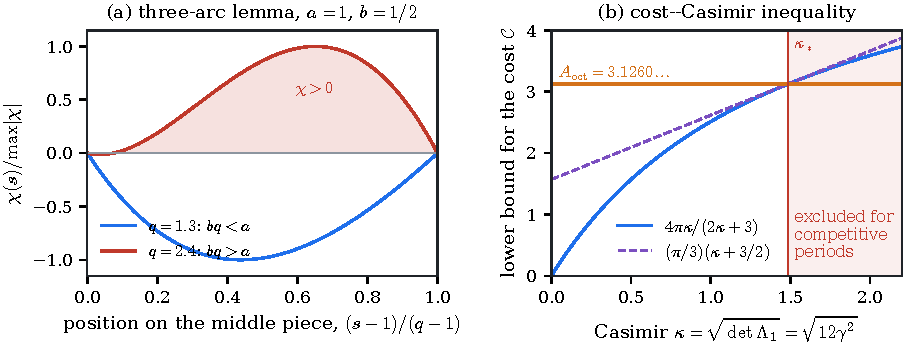
\includegraphics[width=\textwidth]{figures/fig-reverse-estimates.pdf}
  \caption{(a) The obstruction of the three-arc lemma (\cref{lem:three-arc}), growing case, with
  active margin $a=1$ of the middle piece and outer margin $b=a_k=1/2$. The switching function
  of the outer label vanishes at both ends of the middle piece, and its value inside is fixed
  by this. For $q=4/3$ ($bq<a$) it is negative, as the maximum principle requires; for $q=5/2$
  ($bq>a$, that is, $a_ka_{k+2}>a_{k+1}^2$) it becomes positive. The curves are normalized by
  their maximum modulus. (b) The cost--Casimir inequality of \cref{prop:cost-casimir} (solid) and
  the spectral bound of forward periods (dashed), against the octagon's cost $\Aoct$. A
  competitive period has $\kappa<\kappa_*=3\Aoct/(4\pi-2\Aoct)$; the proof of
  \cref{cor:casimir-cap} compares it with $2\sqrt5/3$. Both bounds equal $\pi$ at
  $\kappa=3/2$.}
  \label{fig:reverse-estimates}
\end{figure}
